\scanpage{118}
\fbox{\uline{Corollaire} Soit $U$ une partie ouverte de $\operatorname{Spec}(A)$ contenant $\operatorname{Spec}(A_f)$ et les $p_i$,}

\uline{Corollaire 1} Soit $X$ un schéma \uline{affine} sur $A$, et $s$ une section rationnelle de $X/A$, définie dans $\operatorname{Spec}(A_f)$ et aux points $p_i$. Alors $s$ est définie partout.
\figure{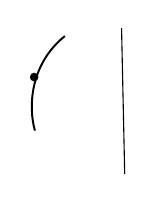
\begin{tikzpicture}[x=1cm,y=1cm]
\draw[line width=.7pt] (.48,1.2) .. controls (.02,.83) and (.02,.27) .. (.1,0);
\fill (.09,.68) circle (.055);
\draw (1.2,1.3)--(1.24,-.55);
\end{tikzpicture}}

Faisant $X=\operatorname{Spec} A[T,T^{-1}]$, on trouve

\uline{Corollaire 2} $A^*=A_f^*\cap\displaystyle\bigcap_i A_{p_i}^*$.

On peut \unsure{énoncer ceci} en disant qu'on a une \inserted{suite exacte de groupes}
\diagram{\begin{tikzcd}[column sep=1.15em,row sep=1.8em]
0 \arrow[r] & A^* \arrow[r] & A_f^* \arrow[r] & \deleted{\unsure{\prod}}\mathbf{Z}^I \arrow[r] & \mathbf{Z}^{\textcircled{\scriptsize I}} \\
&& \figure{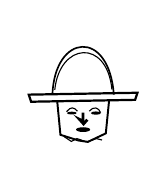
\begin{tikzpicture}[x=.6cm,y=.6cm,baseline=0]
\draw[line width=.6pt] (-.65,.4) .. controls (-.6,1.7) and (.55,1.8) .. (.65,.4);
\draw (-.6,.5) .. controls (-.5,1.5) and (.5,1.6) .. (.61,.51);
\draw[line width=.8pt] (-1.15,.4)--(1.15,.44)--(1.1,.29)--(-1.1,.25)--cycle;
\draw[line width=.7pt] (-.55,.28)--(-.48,-.45)--(-.1,-.57)--(.1,-.6)--(.48,-.42)--(.55,.28);
\draw (-.35,.04) .. controls (-.26,.15) and (-.2,.14) .. (-.12,.05);
\fill (-.24,.01) ellipse (.105 and .03);
\draw (.13,.05) .. controls (.22,.16) and (.33,.13) .. (.37,.02);
\fill (.27,.01) ellipse (.105 and .035);
\draw[line width=1pt] (0,.02)--(0,-.16)--(-.08,-.12)--(.01,-.22)--(.09,-.13);
\fill (0,-.34) ellipse (.15 and .05);
\draw (-.4,-.49)--(-.25,-.59)--(-.13,-.53)--(.07,-.6)--(.28,-.53)--(.4,-.56);
\end{tikzpicture}} && \\
& K^*/A^* \arrow[r] \arrow[d] & K^*/A_f^* \arrow[d] && \\
& \mathbf{Z} \arrow[r] & \mathbf{Z}^I && \\
0 \arrow[r] & A^*\times\mathbf{Z} \arrow[r] & A_f^* \arrow[r] & \mathbf{Z}^I & \\
&& A^*\times\mathbf{Z} \arrow[u] \arrow[r,no head] & \mathbf{Z}^{\deleted{\unsure{I}}} \arrow[u] &
\arrow[from=1-1,to=5-2,no head,out=-50,in=105,looseness=1.3]
\arrow[from=1-1,to=4-2,no head,out=-35,in=170,looseness=1.6]
\arrow[from=1-1,to=1-5,no head,bend left=6]
\arrow[from=1-5,to=5-3,no head,out=-50,in=20,looseness=1.2,line width=1pt]
\arrow[from=1-5,to=3-4,no head,out=-85,in=85,looseness=1.6]
\arrow[from=4-3,to=5-3,no head,out=-145,in=80]
\end{tikzcd}}

\uline{Corollaire 3} Supposons $(f)$ \uline{premier}. Alors \deleted{\unsure{A_f^*}} \deleted{et} $A_f^*\simeq A^*\times\mathbf{Z}$, i.e. \deleted{\unsure{tout}} $t\in A_f^*$ s'écrit de façon unique sous la forme $\varepsilon f^n$, $\varepsilon\in A^*$, $n\in\mathbf{Z}$.
\deleted{\unsure{à diviseur premier}}
\margin{117}
